\documentclass[final]{beamer}

\usepackage[size=a2,orientation=portrait,scale=0.80]{beamerposter}
\usepackage{graphicx}
\usepackage{tikz}
\usepackage{xcolor}
\usepackage{hyperref}
\usepackage[most]{tcolorbox}

% -----------------------------------------------------------------------
% Fonts: classic Computer Modern serif
% -----------------------------------------------------------------------
\usefonttheme{serif}
\setbeamerfont{block title}{size=\normalsize, series=\bfseries, family=\rmfamily}
\setbeamerfont{block body}{size=\small, family=\rmfamily}

% -----------------------------------------------------------------------
% Colours — almost monochrome / academic
% -----------------------------------------------------------------------
\definecolor{captioncolor}{RGB}{80,80,80}

\setbeamercolor{background canvas}{bg=white}
\setbeamercolor{block title}{fg=black, bg=white}
\setbeamercolor{block body}{fg=black, bg=white}
\setbeamertemplate{navigation symbols}{}

% -----------------------------------------------------------------------
% Block style: bold title + rule, no coloured box
% -----------------------------------------------------------------------
\setbeamertemplate{block begin}{%
  \vskip0.1cm
  \par\noindent
  {\usebeamerfont{block title}\bfseries\insertblocktitle}%
  \par\noindent\rule{\linewidth}{0.8pt}\par
  \vskip0.12cm
  \usebeamerfont{block body}%
}
\setbeamertemplate{block end}{\par\vskip0.05cm}

% -----------------------------------------------------------------------
% Headline
% -----------------------------------------------------------------------
\setbeamertemplate{headline}{%
  \leavevmode
  \begin{beamercolorbox}[wd=\paperwidth]{headline}
    \begin{tikzpicture}[remember picture]
      \fill[white] (0,0) rectangle (\paperwidth, 5.0cm);
      \node[anchor=west, align=left, text width=0.70\paperwidth,
            font=\rmfamily\bfseries\Large] at (1.3cm, 3.8cm)
        {Simulation of a Computer Game by Diffusion Model};
      \node[anchor=west, align=left, text width=0.70\paperwidth,
            font=\rmfamily\normalsize] at (1.3cm, 2.3cm)
        {Luk\'a\v{s} Foukal \enspace David Nepra\v{s} \enspace Michael Pe\v{s}tuka};
      \node[anchor=west, align=left, text width=0.70\paperwidth,
            font=\rmfamily\small, text=captioncolor] at (1.3cm, 1.4cm)
        {Faculty of Information Technology, Brno University of Technology $\cdot$ May 2026};
      \node[anchor=east] at (\paperwidth - 1.2cm, 3.0cm)
        {
\includegraphics[height=3.6cm]{figures/FIT_color_CMYK_EN.pdf}};
      \draw[line width=1pt] (0, 0.45cm) -- (\paperwidth, 0.45cm);
    \end{tikzpicture}%
  \end{beamercolorbox}%
  \vskip0.35cm
}

% -----------------------------------------------------------------------
% Footline — heatmap lives just above this
% -----------------------------------------------------------------------
\setbeamertemplate{footline}{%
  \begin{beamercolorbox}[wd=\paperwidth]{footline}
    \begin{tikzpicture}[remember picture]
      \fill[white] (0,0) rectangle (\paperwidth, 1.3cm);
      \draw[line width=0.8pt] (0, 1.05cm) -- (\paperwidth, 1.05cm);
      \node[anchor=west, font=\rmfamily\footnotesize, text=captioncolor]
        at (1.3cm, 0.5cm)
        {\href{https://github.com/MichaelPestuka/KNN_proj}%
              {github.com/MichaelPestuka/KNN\_proj}};
      \node[anchor=east, font=\rmfamily\footnotesize, text=captioncolor]
        at (\paperwidth - 1.3cm, 0.5cm)
        {KNN Project $\cdot$ Spring 2026};
    \end{tikzpicture}%
  \end{beamercolorbox}%
}

% -----------------------------------------------------------------------
\begin{document}
\begin{frame}[t]{}

% =======================================================================
% TWO-COLUMN BODY
% =======================================================================
\begin{columns}[T]

% -----------------------------------------------------------------------
\begin{column}{0.47\textwidth}

  \begin{block}{Problem}
    The goal is to create a \textbf{playable, real-time simulation} of a
    computer game using a diffusion model. Given the previous frame sequence
    and the current player action, the model predicts the next frame ---
    effectively replacing the game engine with a neural network.
  \end{block}

  \vskip0.25cm

  \begin{block}{Data Generation}
    Training data was collected from a \textbf{Super Mario Bros.\ emulator}
    using varying strategies, including pre-trained AI systems playing the game. This results in good level coverage (see full-width occupancy heatmap at the bottom of this poster).

    \smallskip
    Early datasets were heavily biased toward \emph{right-moving} actions
    ($<$6\,\% left) and the resulting model suffered from ignoring user input. The 3rd-generation dataset fixed this with a balanced ratio of actions and taken while also including frames where movement actually happened.

    \smallskip
    \begin{center}
      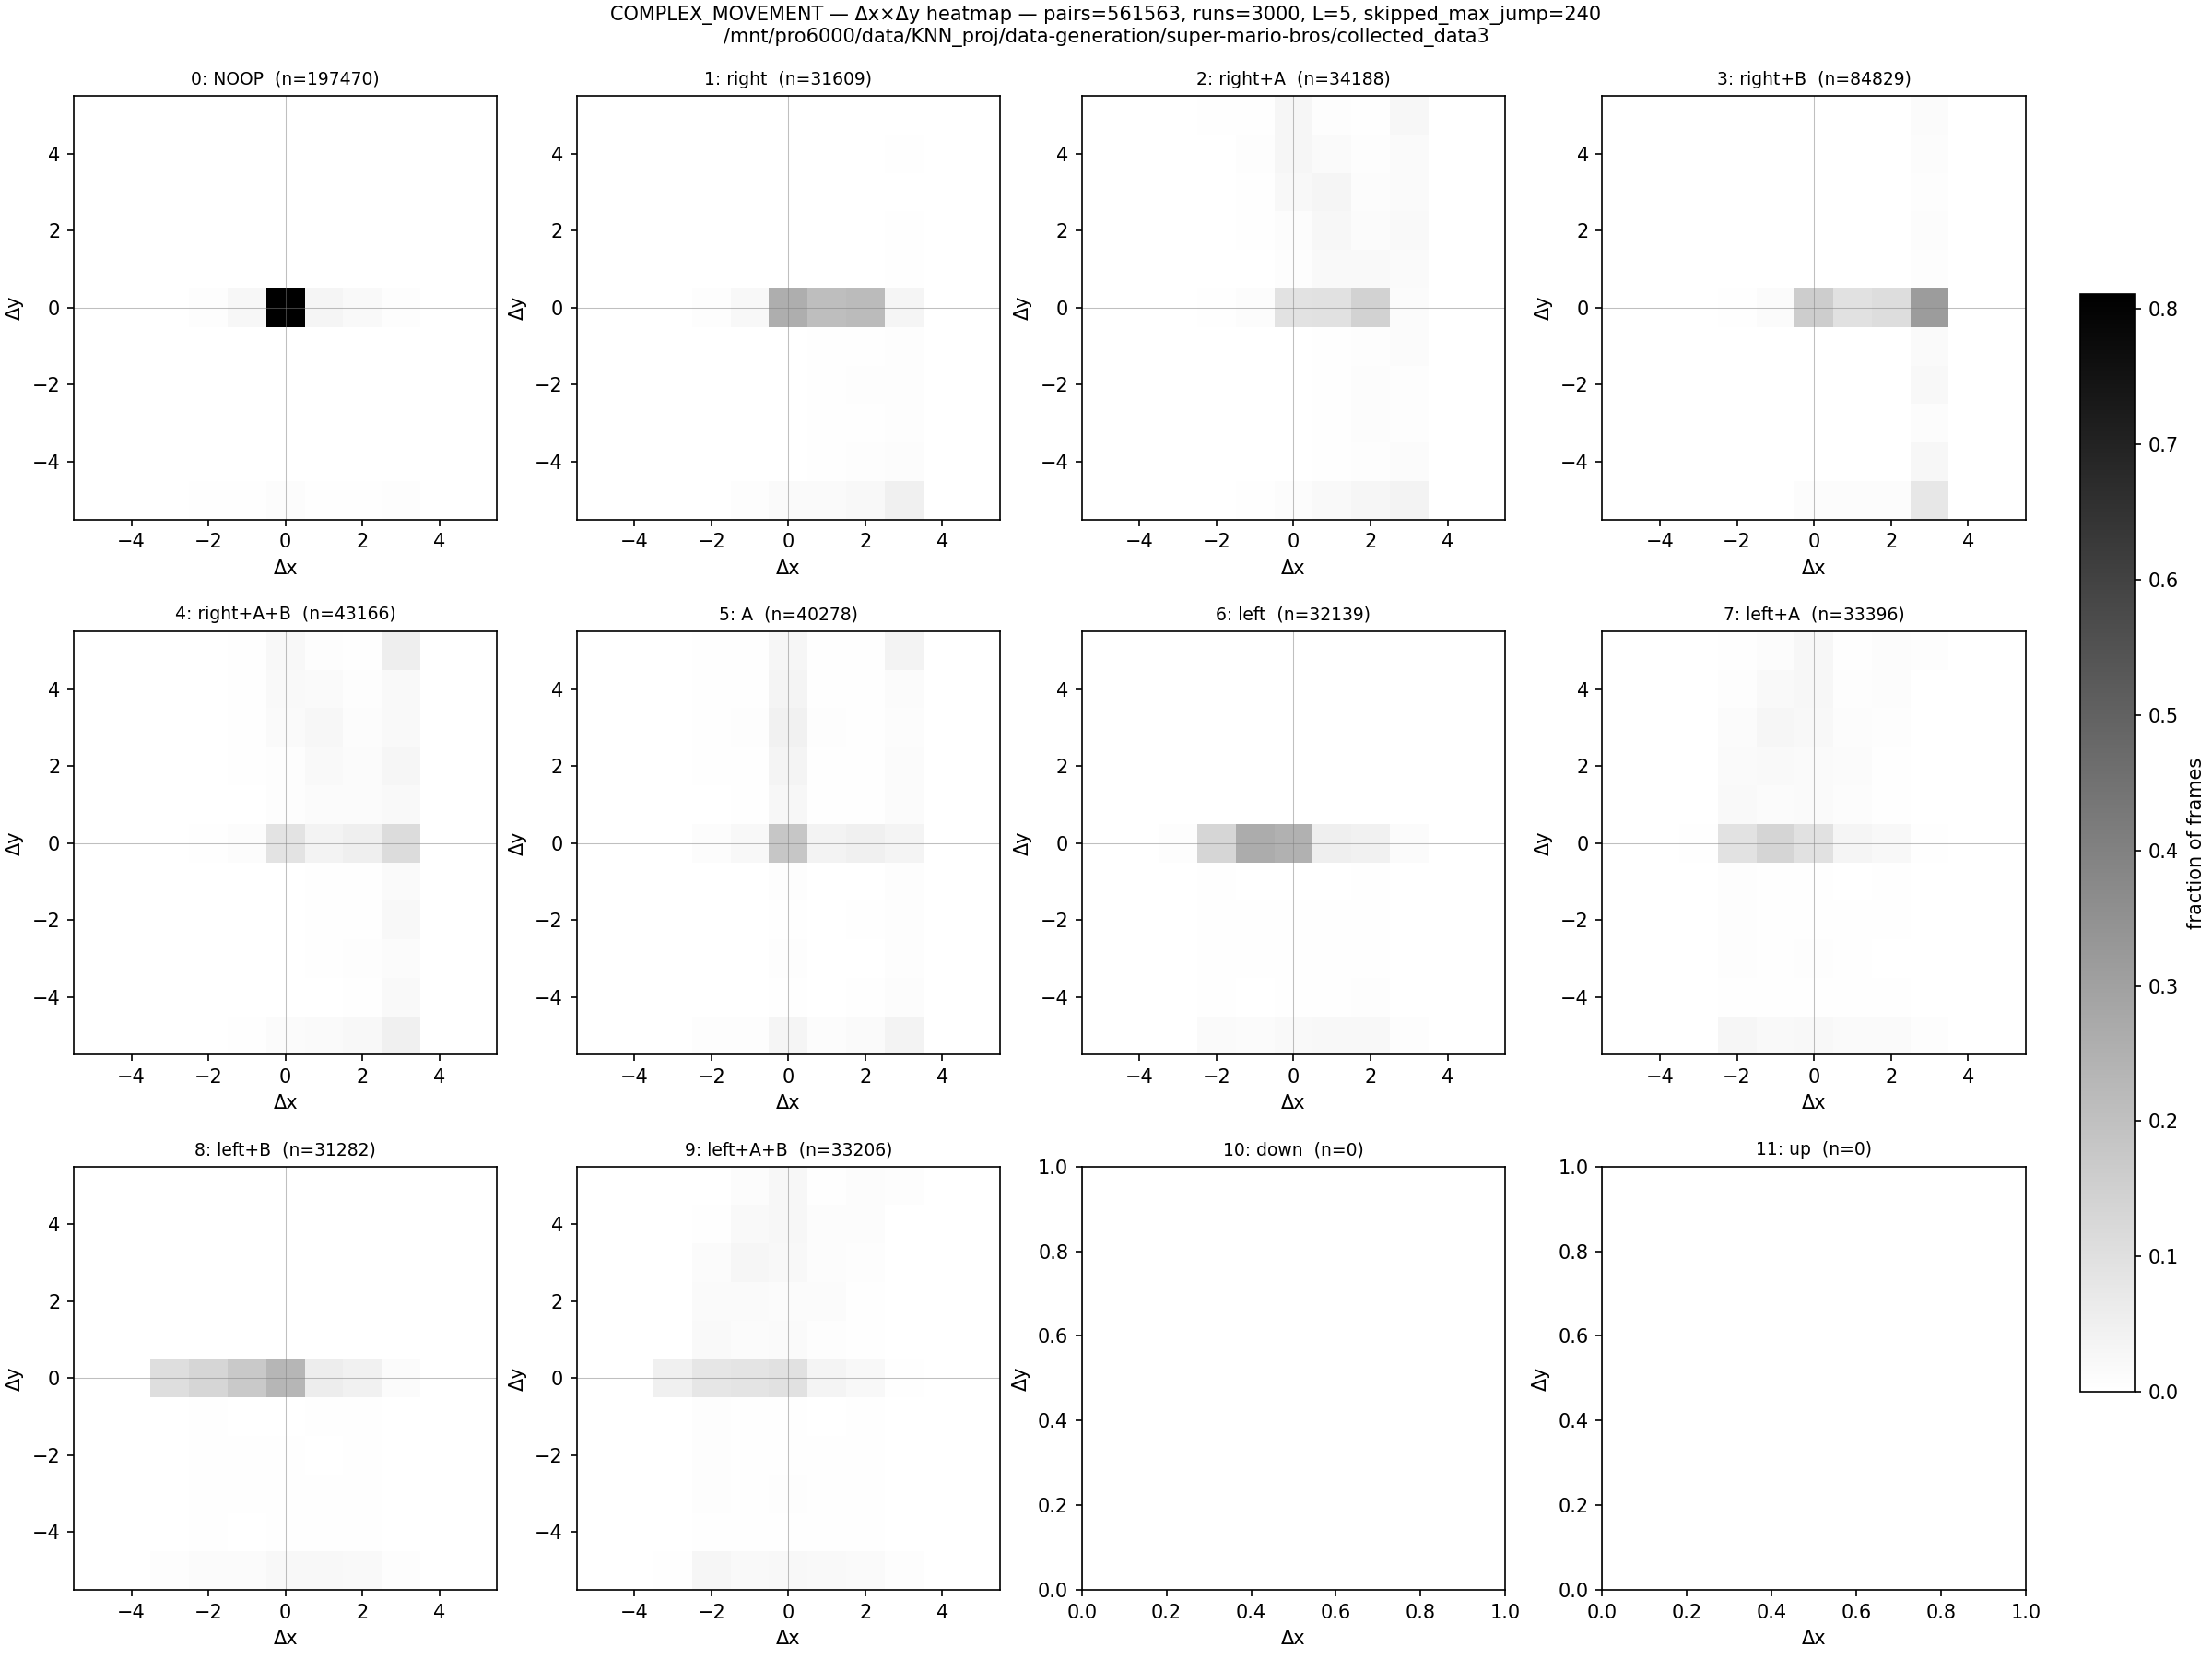
\includegraphics[width=0.90\linewidth]{figures/collected_data3_actions_562k.png}
      \par\vskip2pt
      {\footnotesize\color{captioncolor}%
        Per-action direction maps --- near-uniform action distribution and also clearly visible real movement}
    \end{center}
  \end{block}

  \vskip0.25cm

  \begin{block}{GameNGen Architecture}
    Based on \textbf{Stable Diffusion 1.4}, adapted for game simulation:
    \begin{itemize}\setlength\itemsep{1pt}
      \item Action tokens replace text cross-attention.
      \item Previous frames (VAE-encoded) concatenated to noised latents.
      \item First Conv layer re-initialised to accept $4n$ input channels.
      \item \textbf{Noise augmentation} on context frames prevents drift.
      \item \textbf{Decoder fine-tuning} removes VAE blur artefacts.
    \end{itemize}
    \smallskip
    Based on the open-source GameNGen reproduction by Stiegler et al.
  \end{block}

  \vskip0.25cm

  \begin{block}{Interactive Demo}
    A \textbf{portable Python GUI} streams gameplay over SSH to a remote
    inference server. Player inputs are forwarded; JPEG-encoded frames
    stream back in real time.

    \smallskip
    Optimisations: only \textbf{3 diffusion steps}, FP16
    precision throughout, and VAE decode + JPEG encode offloaded to a
    \textbf{second GPU} keeping the primary GPU on the UNet continuously.

    \smallskip
    \begin{tcolorbox}[colback=gray!7, colframe=black, sharp corners,
                      boxrule=0.6pt, top=3pt, bottom=3pt, left=6pt, right=6pt,
                      fontupper=\rmfamily\small]
      $\approx$\textbf{22.5 FPS} on dual RTX PRO 6000 Blackwell at
      $\sim$300\,W \quad (\textit{live demo at the poster!})
    \end{tcolorbox}
  \end{block}

  \vskip0.25cm

  \begin{block}{Context Length Ablation}
    Models trained separately per context length; the
    \textbf{9-frame context} (matching the original GameNGen paper)
    consistently performs best across both PSNR and LPIPS.

    \smallskip
    \begin{center}
      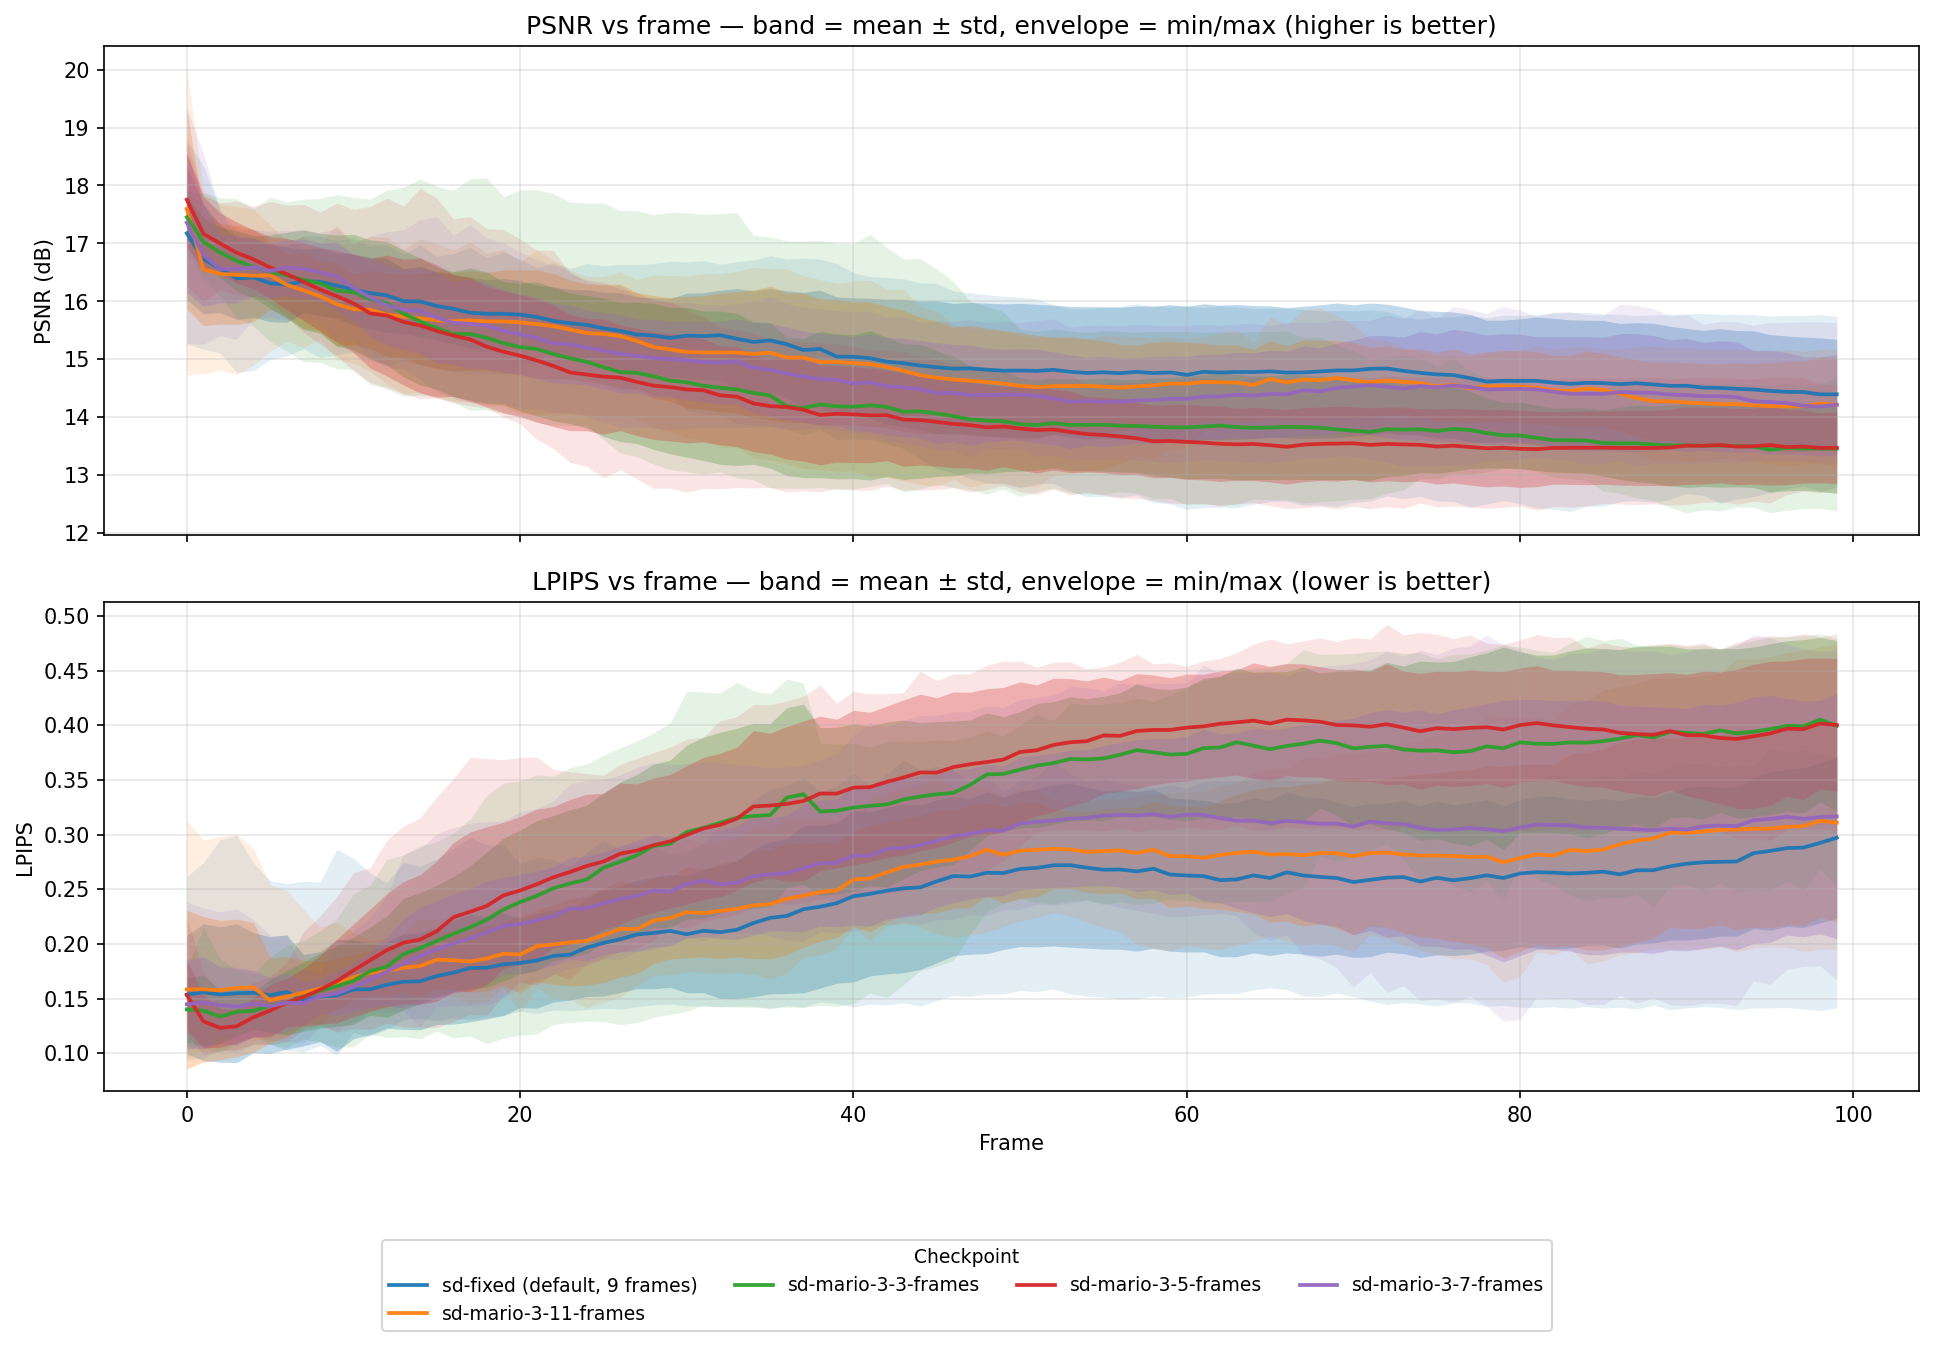
\includegraphics[width=0.90\linewidth]{figures/context_length_compare_human_data.png}
      \par\vskip2pt
      {\footnotesize\color{captioncolor}%
        Aggregated per-frame metrics across varying context lengths (trained on first generation dataset, evaluated on human gameplay data)}
    \end{center}
  \end{block}

\end{column}

\hfill

% -----------------------------------------------------------------------
\begin{column}{0.47\textwidth}

  \begin{block}{ControlNet-Based Approach}
    An alternative pipeline that \textbf{decouples game logic from rendering}:

    \smallskip
    \textbf{1. Transformer World Model} --- processes sequential
    (coordinates, actions, compressed latents) and predicts the next latent.

    \smallskip
    \textbf{2. Decoder $\to$ Segmentation Mask} --- a CNN decoder upsamples
    the latent into a multi-class semantic segmentation map.

    \smallskip
    \textbf{3. ControlNet Renderer} --- Stable Diffusion + semantic ControlNet
    renders the final frame conditioned on the segmentation map.

    \smallskip
    \begin{center}
      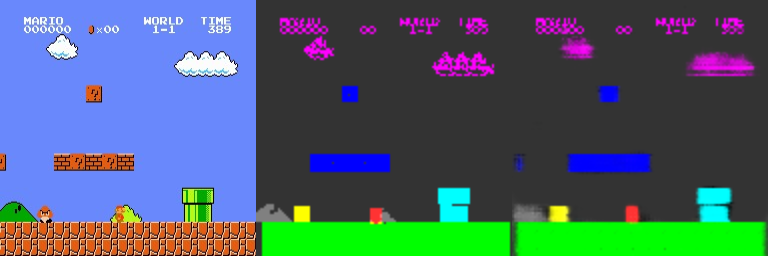
\includegraphics[width=0.94\linewidth]{figures/controlnet_based.png}
      \par\vskip2pt
      {\footnotesize\color{captioncolor}%
        Left: GT RGB.\quad Centre: GT segmentation.\quad Right: Predicted segmentation.}
    \end{center}

    \smallskip
    \textbf{Training highlights:}
    \begin{itemize}\setlength\itemsep{1pt}
      \item \emph{Progressive rollout}: 1-step teacher forcing $\to$
            100-step autoregressive sequences.
      \item \emph{Composite loss}: BCE + soft Dice + Sobel boundary
            + physics-gated spatial loss.
      \item Physics prior centred on the Transformer's predicted coordinates
            enforces spatial consistency.
    \end{itemize}
  \end{block}

  \vskip0.25cm

  \begin{block}{Evaluation}
    Metrics: \textbf{PSNR} and \textbf{LPIPS}
    (Learned Perceptual Image Patch Similarity).
    Ground truth is instrumented human gameplay.

    \smallskip
    \begin{center}
      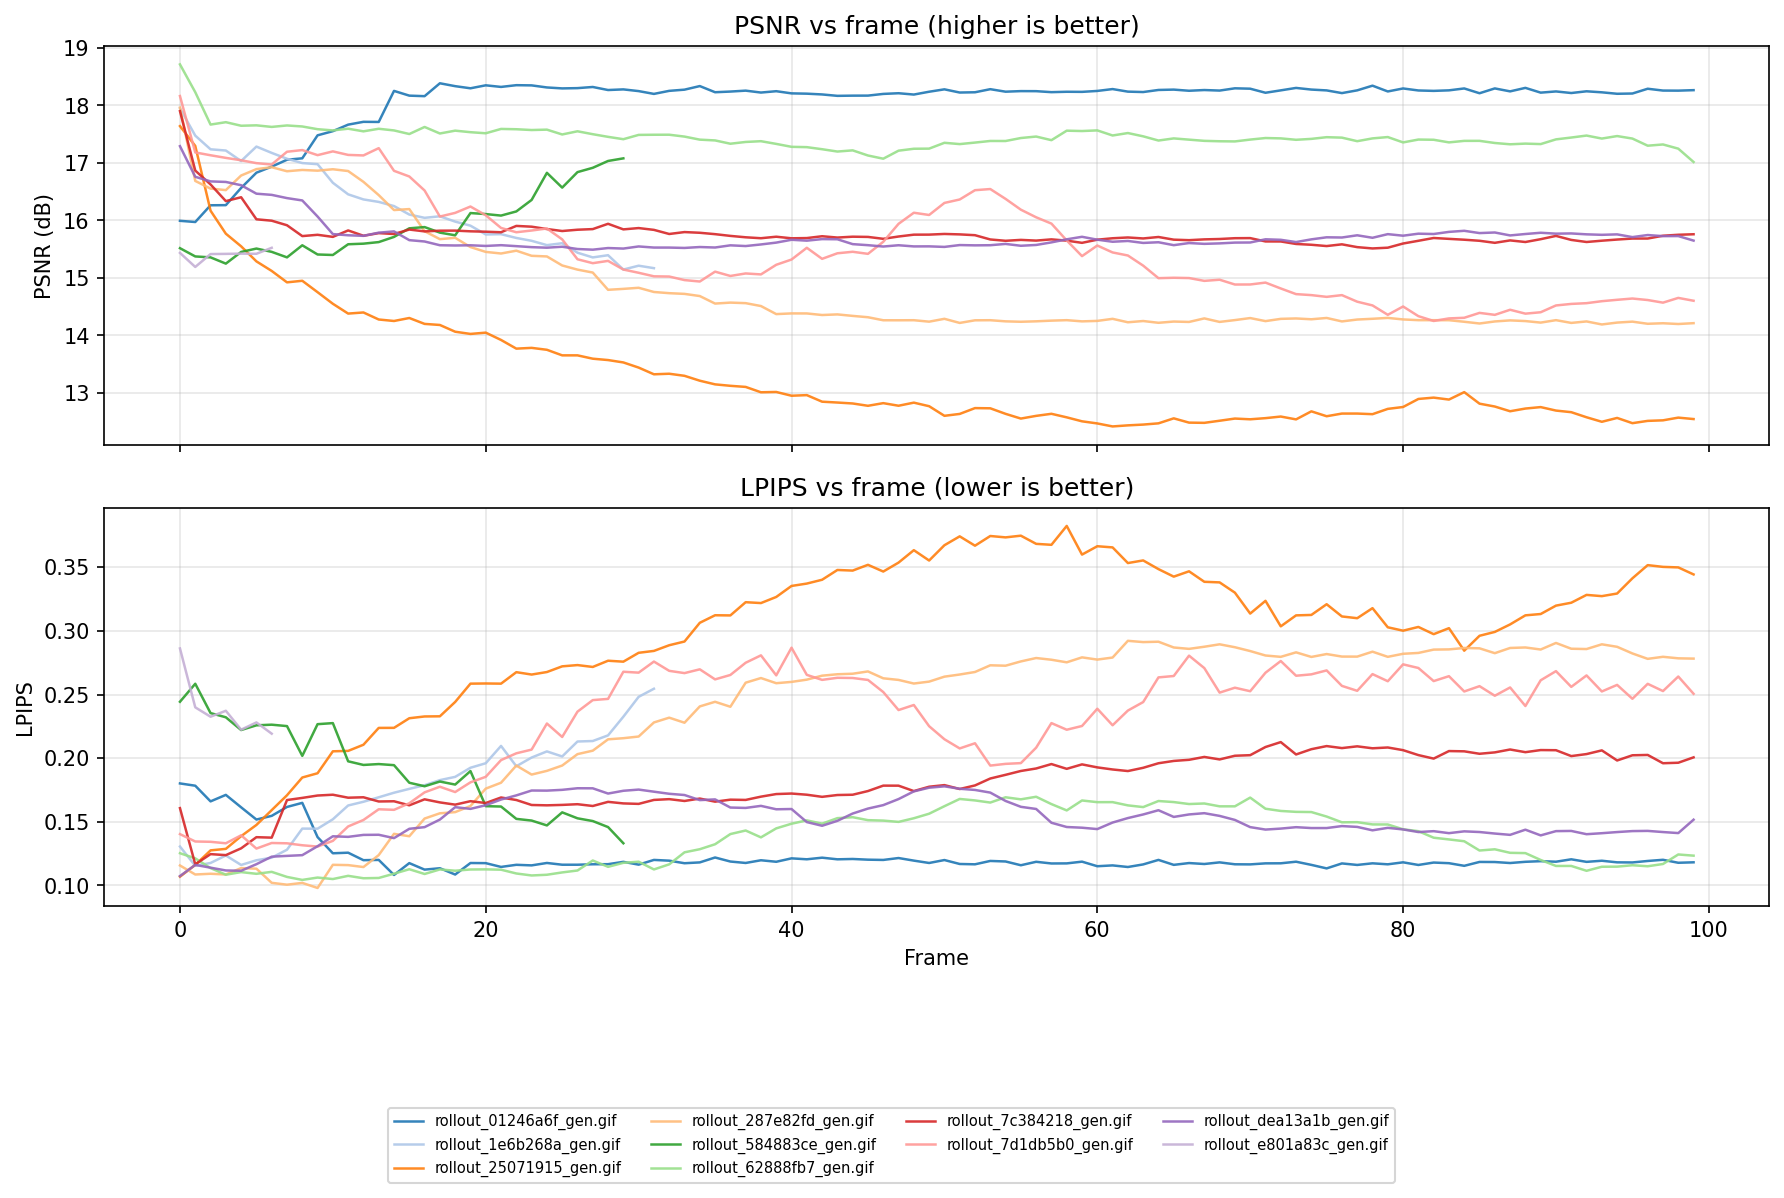
\includegraphics[width=0.92\linewidth]{figures/sd-mario-3_human_data.png}
      \par\vskip2pt
      {\footnotesize\color{captioncolor}%
        Per-frame metrics on 10 human gameplay sequences
        (\texttt{sd-mario-3}, 3 diffusion steps)}
    \end{center}

    \smallskip
    \begin{center}
      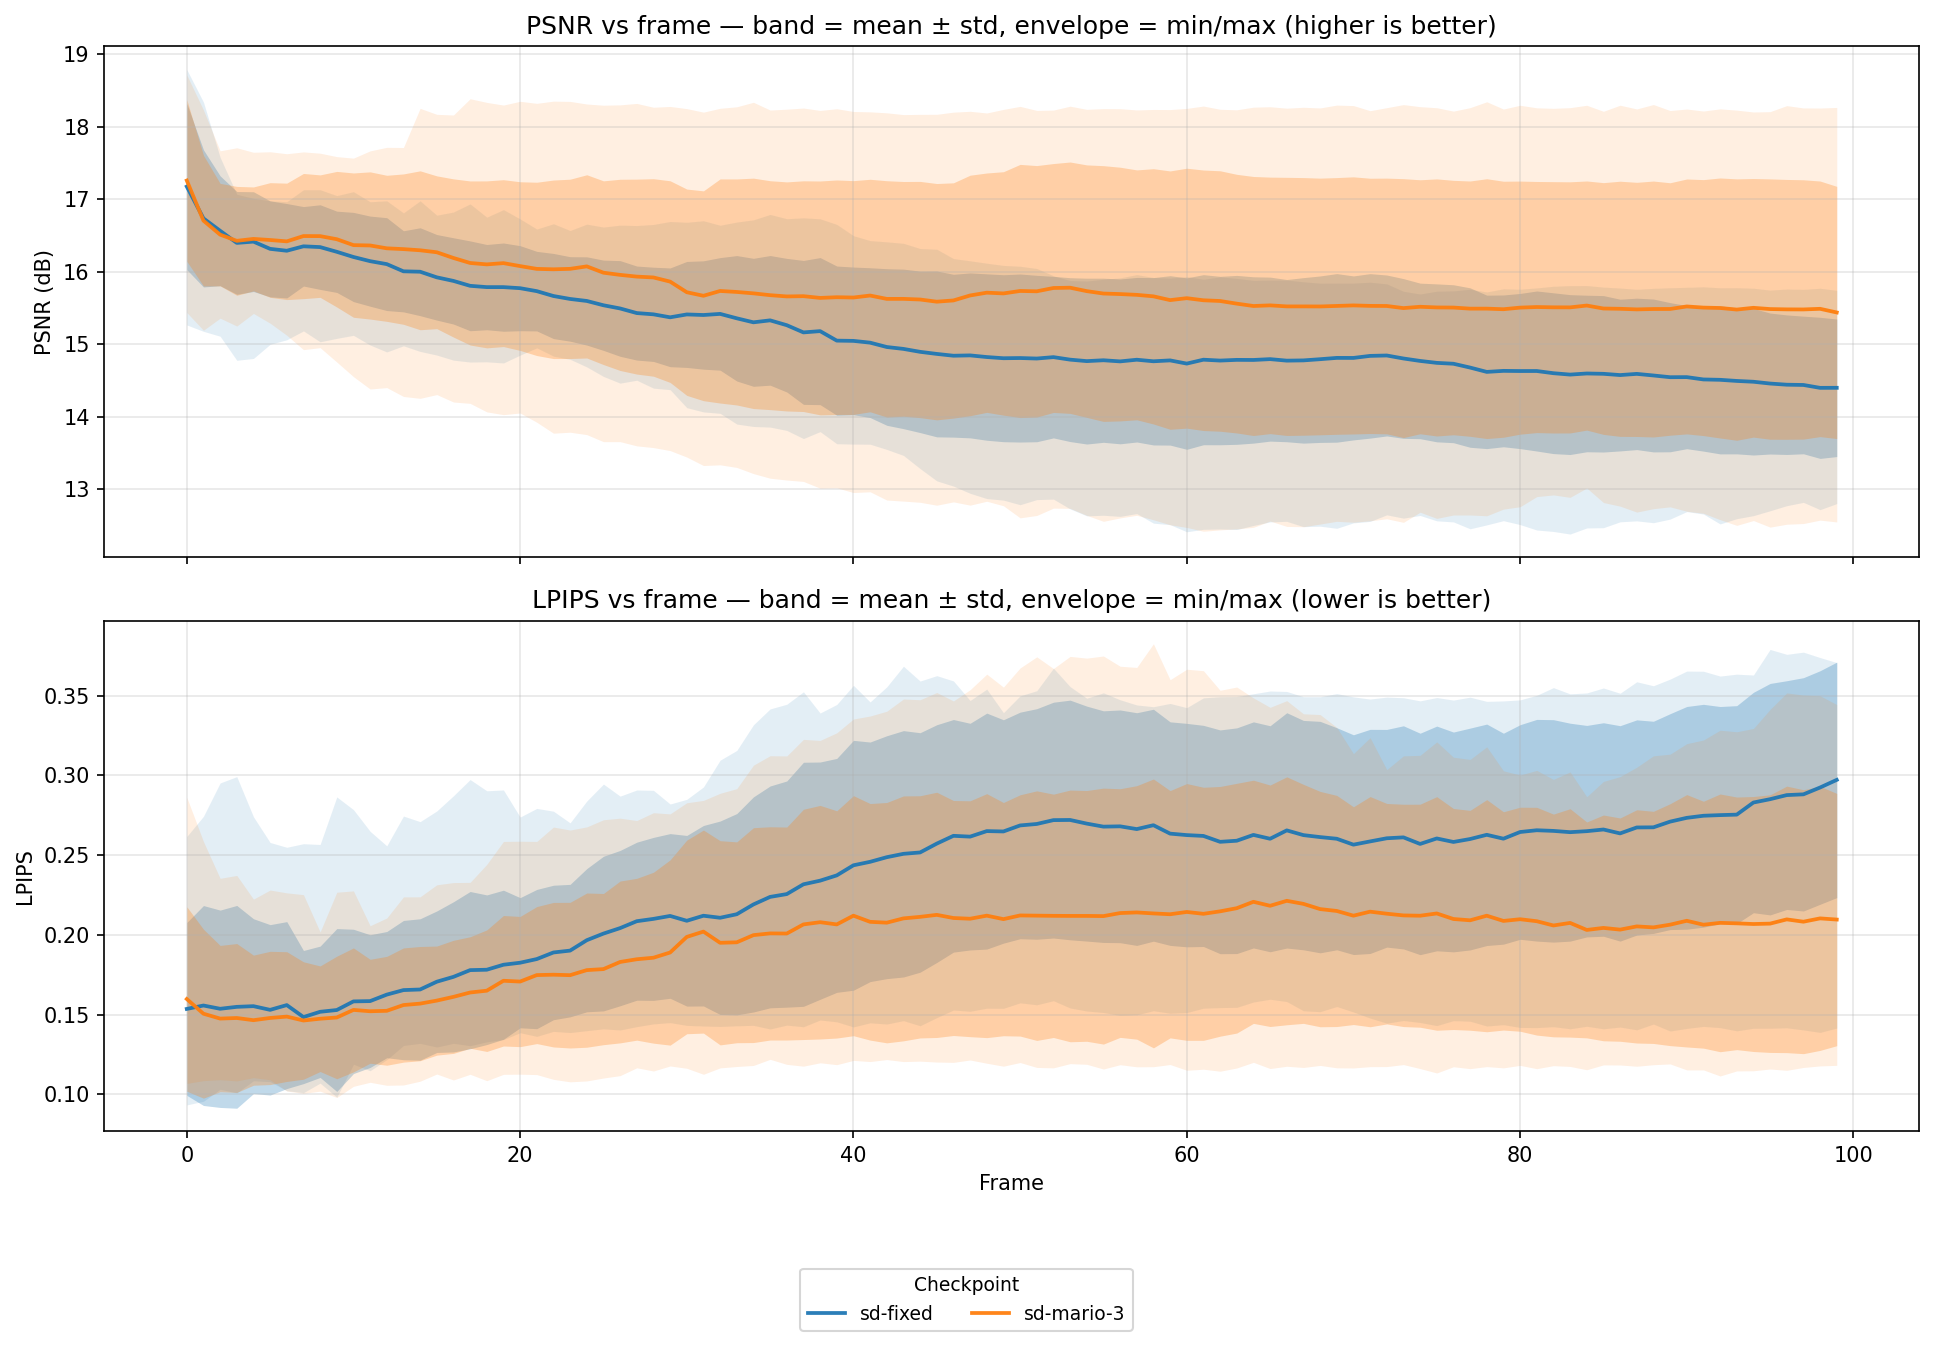
\includegraphics[width=0.92\linewidth]{figures/data_compare_eval_1&3.png}
      \par\vskip2pt
      {\footnotesize\color{captioncolor}%
        \texttt{sd-fixed} (checkpoint) vs.\ \texttt{sd-mario-3} (latest) ---
        improved data yields clearly better metrics}
    \end{center}

    \smallskip
    \begin{tcolorbox}[colback=gray!7, colframe=black, sharp corners,
                      boxrule=0.6pt, top=3pt, bottom=3pt, left=6pt, right=6pt,
                      fontupper=\rmfamily\small]
      \textbf{Key result:} \texttt{sd-mario-3} at 3 diffusion steps achieves
      \textbf{better LPIPS than original GameNGen at 4 steps} Important to keep in mind that this game is less complex. There may also be other differences in our methodology.
    \end{tcolorbox}
  \end{block}

\end{column}

\end{columns}

% =======================================================================
% FULL-WIDTH HEATMAP — bottom of poster
% =======================================================================
\vfill
\vskip0.3cm
{\rmfamily\bfseries\normalsize World 1-1 Occupancy Heatmap}
\par\noindent\rule{\textwidth}{0.8pt}
\vskip0.1cm
\begin{center}
  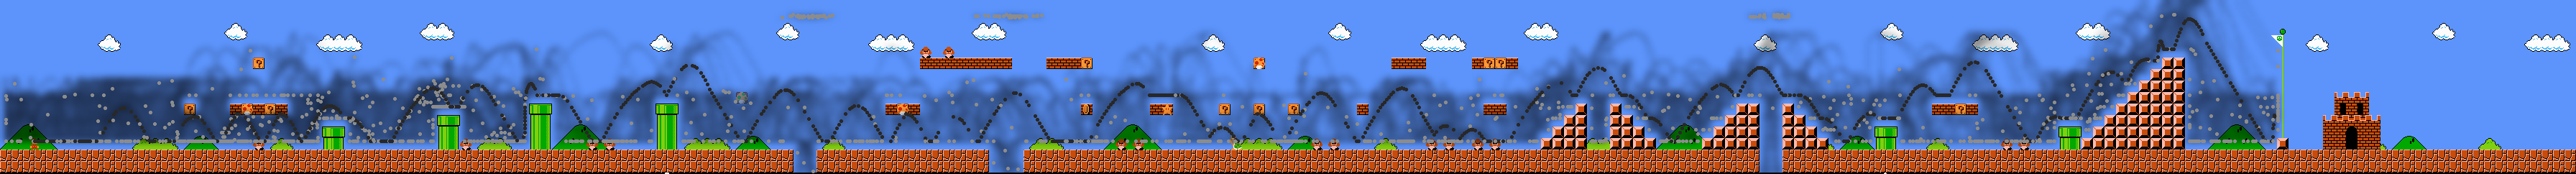
\includegraphics[width=\textwidth]{figures/collected_data3_all_runs_heatmap_562k.png}
  \par\vskip2pt
  {\footnotesize\color{captioncolor}%
    3rd-gen dataset: player position heatmap aggregated across all runs
    (561\,563 logged frames). Black dots show run start positions.}
\end{center}

\end{frame}
\end{document}
